%*************************************************************************
\section{Erstellen eines Technical Difference Builders}\label{sec:TechnicalDifferenceBuilder}
%*************************************************************************

Ein Matcher kann i.d.R. für mehrere Modelle unterschiedlichen Typs benutzt werden. Dahingegen muss für jeden Modelltyp (Metamodell) ein separater \textit{Technical Difference Builder} erzeugt werden.\\
Erstellen Sie dazu über \texttt{File} $\triangleright$ \texttt{New} $\triangleright$ \texttt{Other...}: \texttt{Plug-in Development} $\triangleright$ \texttt{Plug-in Project} eines neues Plugin und öffnen Sie die \texttt{MANIFEST.MF}.
Wechseln Sie auf den Reiter \texttt{Dependencies} und fügen Sie die in Abbildung \ref{silift-plugin_techbuilder_manifest_dependencies} gelisteten Abhängigkeiten hinzu.

\begin{figure}[H]
\centering
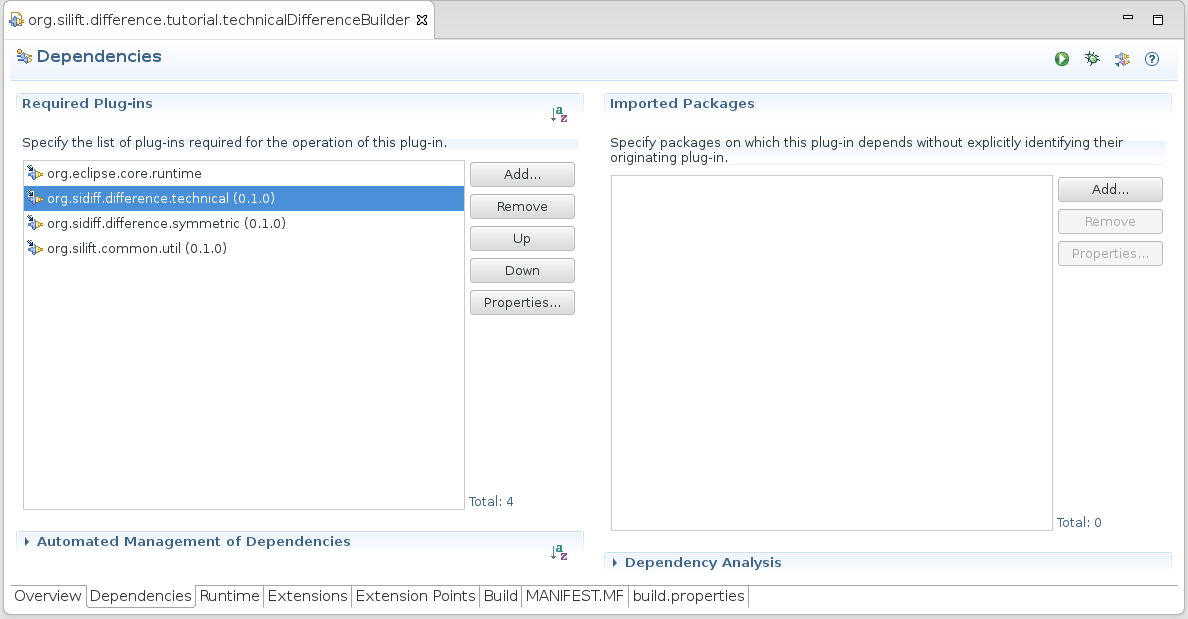
\includegraphics[width=0.8\textwidth]{techbuilder/graphics/silift-plugin_techbuilder_manifest_dependencies.png}
\caption{\texttt{\texttt{MANIFEST.MF} $\triangleright$ \texttt{Dependencies}}}
\label{silift-plugin_techbuilder_manifest_dependencies}
\end{figure}

Als nächstes wird eine Klasse benötigt die die Schnittstelle \texttt{ITechnicalDifferenceBuilder} implementiert (vgl. Abb. \ref{silift-plugin_techbuilder_itechbuilder}).

\begin{figure}[H]
\centering
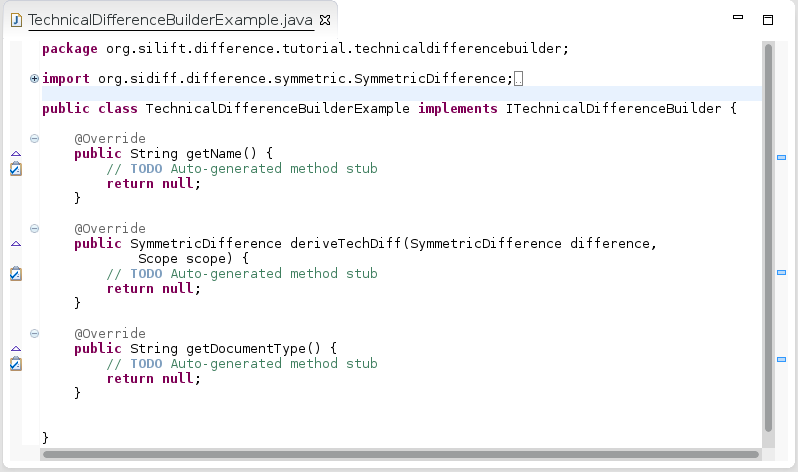
\includegraphics[width=0.6\textwidth]{techbuilder/graphics/silift-plugin_techbuilder_itechbuilder.png}
\caption{Klasse \texttt{TechnicalDifferenceBuilderExample} implementiert \texttt{ITechnicalDifferenceBuilder}}
\label{silift-plugin_techbuilder_itechbuilder}
\end{figure}

Anstatt die Schnittstelle \texttt{ITechnicalDifferenceBuilder} von Grund auf zu implementieren, kann auch die ``Convenience''-Klasse \texttt{Technical\-Difference\-Builder} erweitert werden.\\
Diese implementiert bereits die Methode \texttt{deriveTechDiff}. Durch die manuelle Implementierung der Methoden \texttt{getUnconsideredNodeTypes}, \texttt{getUnconsideredEdgeTypes} und \texttt{getUnconsideredAttributeTypes} können zudem Modellelemente gefiltert und somit von der Differenzbildung ausgeschlossen werden (vgl. Abb. \ref{silift-plugin_techbuilder_techbuilder}).


\begin{figure}[H]
\centering
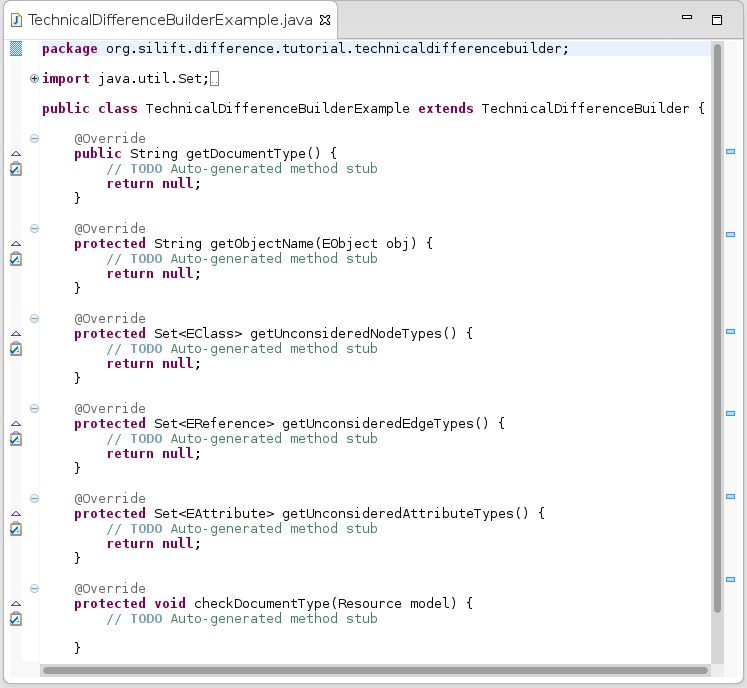
\includegraphics[width=0.6\textwidth]{techbuilder/graphics/silift-plugin_techbuilder_techbuilder.png}
\caption{\texttt{Klasse \texttt{TechnicalDifferenceBuilderExample} erweitert \texttt{TechnicalDifferenceBuilder}}}
\label{silift-plugin_techbuilder_techbuilder}
\end{figure}

Danach muss das Plugin analog zu Abschnitt \ref{sec:own_matching_engine} noch als Extension für \texttt{SiLift} definiert werden.
Gehen Sie dazu wieder in die \texttt{MANIFEST.MF} und wechseln Sie auf den Rei\-ter \texttt{Extensions}. Klicken Sie auf auf \texttt{Add...} und selektieren Sie den \textit{Extension Point} \texttt{org.sidiff.difference.technical.technical\_difference\_builder\_extension} .\\
Klicken sie danach mit der rechten Maustaste auf die Extension und wählen sie \texttt{New} $\triangleright$ \texttt{technical} (vgl. Abb. \ref{silift-plugin_techbuilder_manifest_extension_point}).

\begin{figure}[H]
\centering
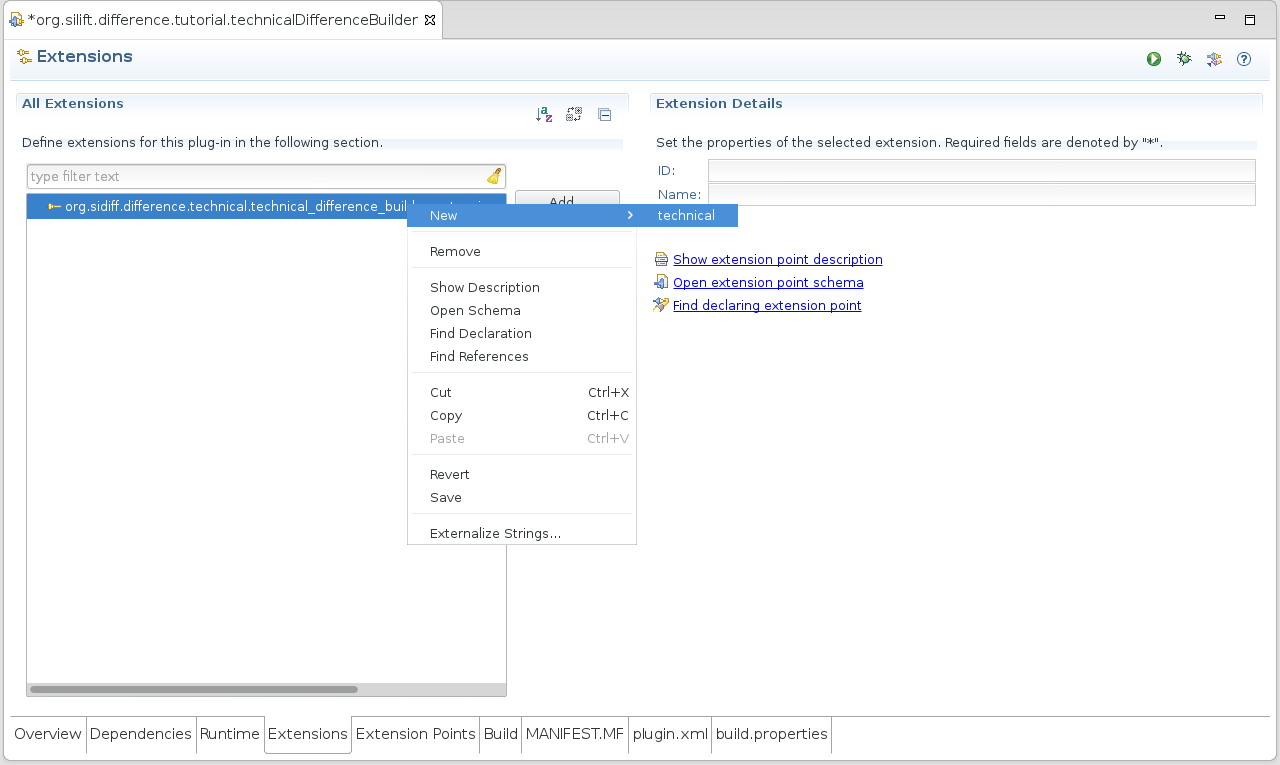
\includegraphics[width=0.8\textwidth]{techbuilder/graphics/silift-plugin_techbuilder_manifest_extension_point.png}
\caption{\texttt{Klasse \texttt{MANIFEST.MF} $\triangleright$  \texttt{Extensions}}}
\label{silift-plugin_techbuilder_manifest_extension_point}
\end{figure}

Als letztes müssen Sie noch unter \texttt{Extension Element Details} $\triangleright$ \texttt{difference\_builder} Ihre zuvor erstellte Klasse eingeben (vgl. Abb. \ref{silift-plugin_techbuilder_manifest_dependencies}).

\begin{figure}[H]
\centering
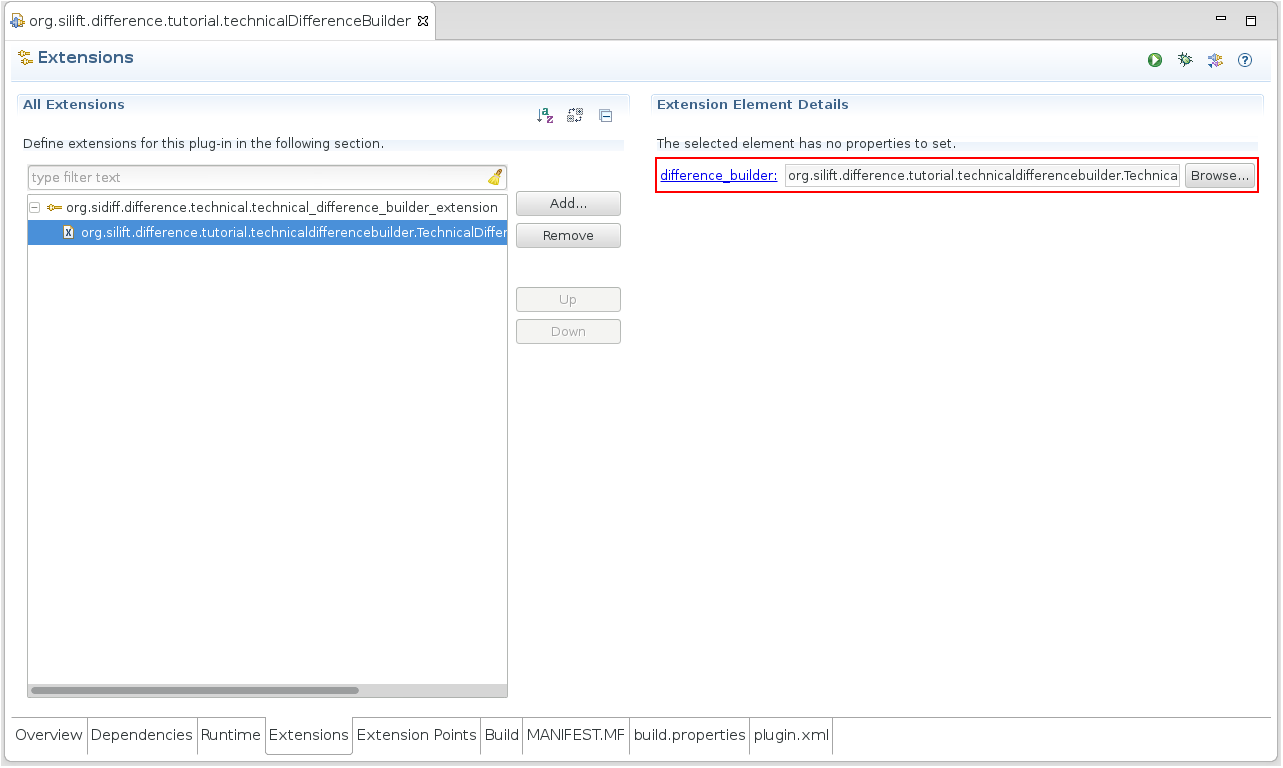
\includegraphics[width=0.8\textwidth]{techbuilder/graphics/silift-plugin_techbuilder_manifest_extension.png}
\caption{\texttt{Klasse \texttt{MANIFEST.MF} $\triangleright$  \texttt{Extensions}: \texttt{difference builder}}}
\label{silift-plugin_techbuilder_manifest_extension}
\end{figure}

Damit SiLift Ihren Difference Builder findet muss dieser noch analog zu Abschnitt \ref{sec:own_matching_engine} deployed werden.
